\documentclass{beamer}
\usepackage{graphicx}
\usepackage{caption}

\title{QuComm: Optimizing Collective Communication for DQC}
\author{Wu, Ding (UCSB), Li (PNNL)}
\date{\today. based on the MICRO 2023 paper}

\begin{document}
	
	\frame{\titlepage}
	
	\begin{frame}{Background: DQC Architecture and Communication Challenges}
		\begin{figure}
			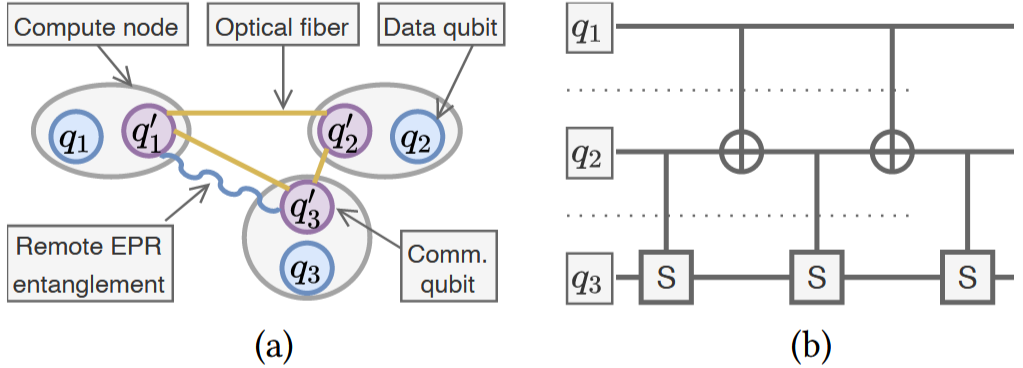
\includegraphics[width=0.8\textwidth]{figure/setup.png}
			\caption[short text]{Common DQC setup. Data qubits handle computation; comm qubits generate EPR pairs.}
		\end{figure}

		\begin{itemize}
			\item Distributed computing uses remote EPR entanglement.
			\item Inter-node communication is expensive and error-prone.
%			\item Goal: Reduce inter-node gate count via compiler techniques.
		\end{itemize}
	\end{frame}
	
	\begin{frame}{Background: Communication Protocols}
		\begin{figure}
			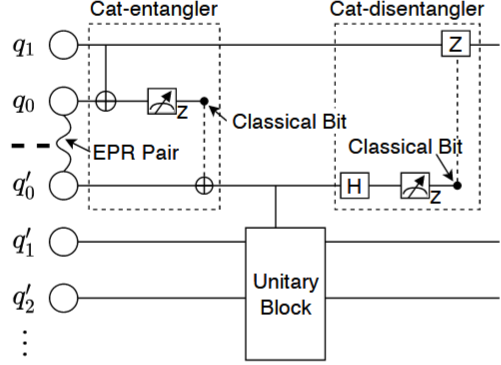
\includegraphics[width=0.4\textwidth]{figure/cat-comm.png}
			\hspace*{4pt}
			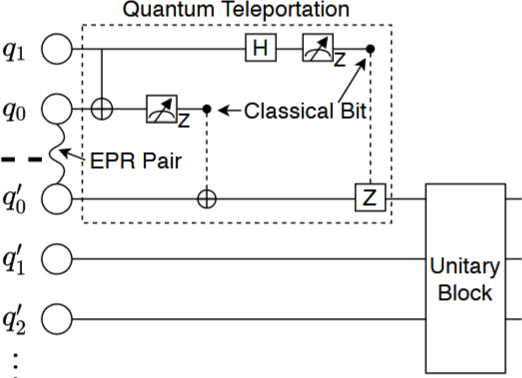
\includegraphics[width=0.4\textwidth]{figure/TP-comm.png}
			\caption{(a) Cat-Comm shares a qubit state; (b) TP-Comm moves it entirely.}
		\end{figure}
		
		\begin{itemize}
			\item Cat-Comm: Efficient for read-only use of shared qubits.
			\item TP-Comm: Required if qubit must be modified.
			\item Each consumes 1 EPR pair.
		\end{itemize}
	\end{frame}
	
	\begin{frame}{QuComm: Overview}
		\begin{itemize}
			\item Goal: Reduce costly inter-node communication in Distributed Quantum Computing (DQC).
			\item Key Idea: Identify and optimize \emph{collective communication} patterns involving multiple nodes.
			\item Authors: Wu, Ding (UCSB), Li (PNNL)
		\end{itemize}
	\end{frame}
	
	\begin{frame}{What is Collective Communication?}
		\begin{itemize}
			\item \textbf{Definition:} A group of inter-node gates involving multiple nodes whose qubit interaction graph is connected.
			\item \textbf{Goal:} Execute all gates in the group together to reduce total inter-node communications.
			\item \textbf{Benefit:} Significant savings — e.g., 5 CNOTs across 3 nodes can use just 2 EPRs if optimized collectively.
			\item \textbf{Challenges:}
			\begin{itemize}
				\item Hidden in low-level gates.
				\item Nontrivial to route and support on limited hardware.
			\end{itemize}
		\end{itemize}
	\end{frame}
	
	\begin{frame}{Motivation: Limitations of Current DQC Compilers}
		\begin{figure}
			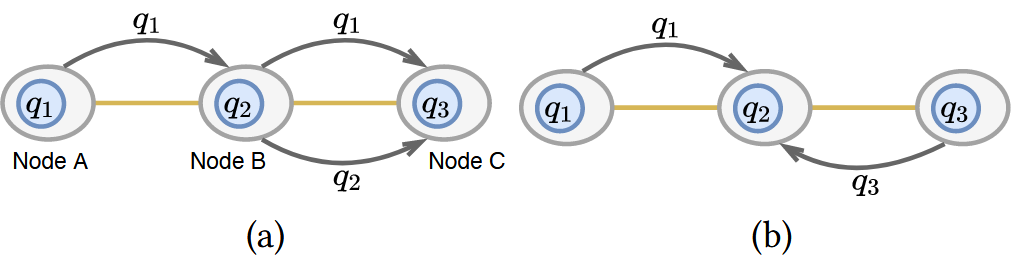
\includegraphics[width=0.85\textwidth]{figure/routing.png}
			\caption[]{Two examples of routing the collective communication block.}
		\end{figure}
		\begin{itemize}
			\item Existing compilers treat inter-node gates independently.
			\item Miss opportunities to group multi-node gates.
			\item QuComm reduces comms by executing groups collectively.
		\end{itemize}
	\end{frame}

	
	\begin{frame}{Method: QuComm Compilation Pipeline}
		\begin{figure}
			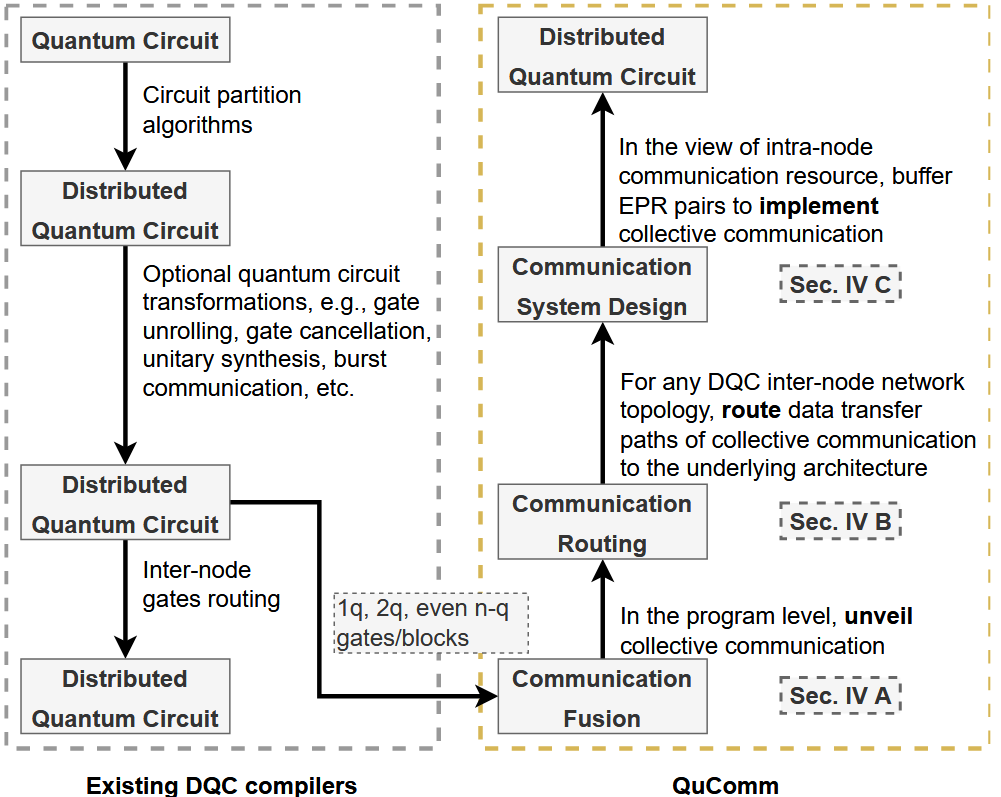
\includegraphics[width=.5\textwidth]{figure/method.png}
			\caption[]{Compilation flow.}
		\end{figure}
		\begin{itemize}
			\item Stage 1: Communication Fusion
			\item Stage 2: Communication Routing
			\item Stage 3: Communication Buffering
		\end{itemize}
	\end{frame}
	
	\begin{frame}{Stage 1: Communication Fusion}
		\begin{figure}
			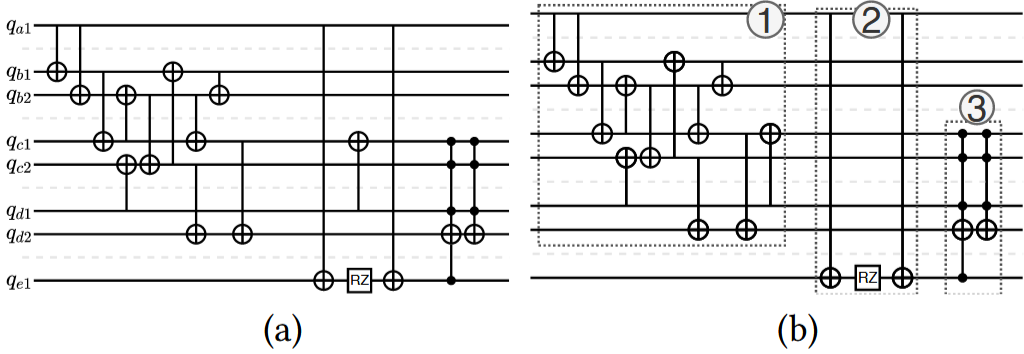
\includegraphics[height=20ex]{figure/step1.png}
			\caption[]{Scattered inter-node gates merged into one collective block, where each node’s EPR capacity is 5.}
		\end{figure}
		\begin{itemize}
			\item Identify and group overlapping multi-node gates.
			\item Merge if group execution reduces communication cost.
			\item Result: Fewer, more efficient collective blocks.
		\end{itemize}
	\end{frame}
	
	\begin{frame}{Stage 2: Routing}
		\begin{figure}
			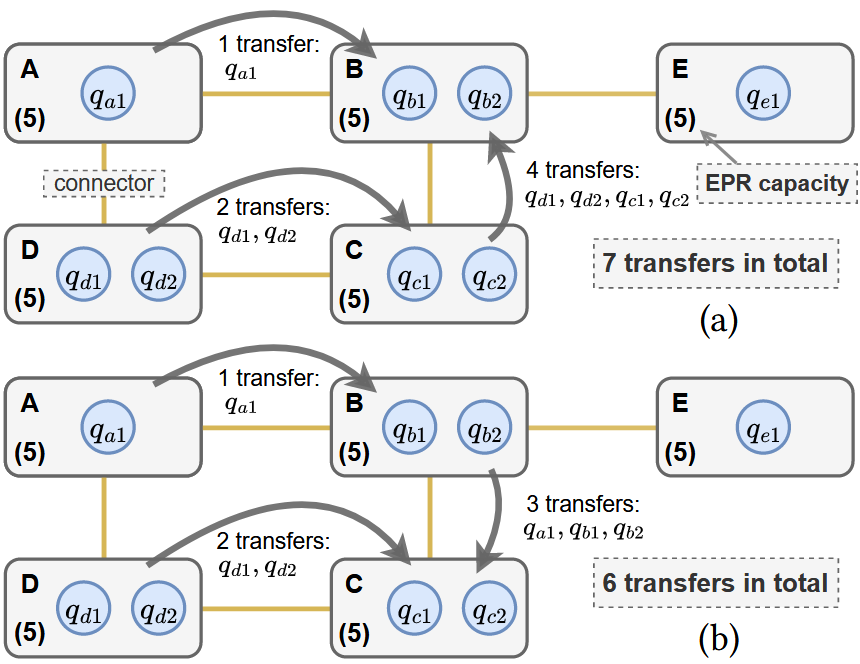
\includegraphics[height=25ex]{figure/step2-1.png}
		\end{figure}
		\begin{itemize}
			\item Select optimal aggregation node.
			\item Design shortest paths with early gate execution.
		\end{itemize}
	\end{frame}
	
	\begin{frame}{Stage 2: Routing}
		\begin{figure}
			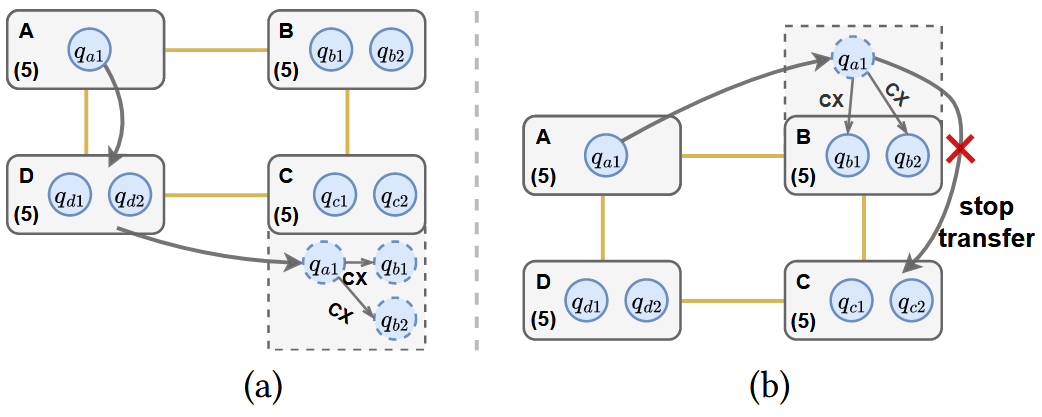
\includegraphics[height=20ex]{figure/step2-2.png}
		\end{figure}
		\begin{itemize}
			\item Select optimal aggregation node.
			\item Design shortest paths with early gate execution.
		\end{itemize}
	\end{frame}
	
	\begin{frame}{Stage 3: Communication Buffering}
		\begin{itemize}
			\item \textbf{Problem:} Not enough comm qubits for large blocks.
			\item \textbf{Solution:} Use spare data qubits to buffer EPR pairs.
			\item \textbf{Result:} Enables large block execution with limited resources.
			\item Only add buffer when it reduces overall cost.
		\end{itemize}
	\end{frame}
	
	\begin{frame}{Evaluation Overview}
		\begin{itemize}
			\item Benchmarks: XOR, RCA, QFT, Grover, etc.
			\item Baseline: AutoComm, GP-CAT, GP-SWAP
			\begin{itemize}
				\item \textbf{AutoComm:} state-of-the-art DQC compiler prior to QuComm
				\item GP-CAT: Uses only Cat-Comm
				\item GP-SWAP: Swaps qubits into place
			\end{itemize}
			\item Metric: Number of inter-node communication ops
		\end{itemize}
	\end{frame}
	
	\begin{frame}{Comparison to AutoComm}
		\begin{figure}
			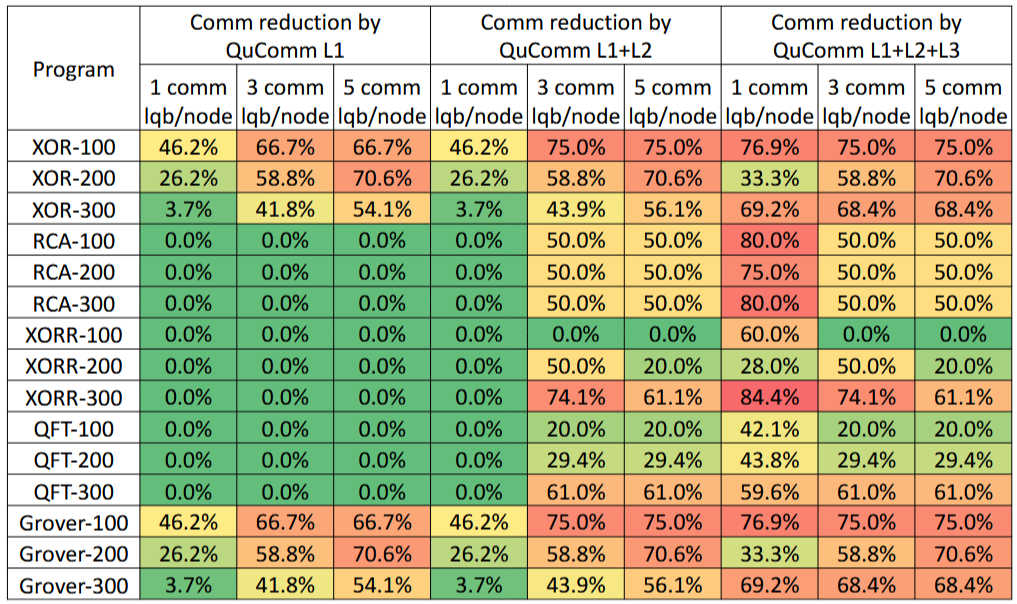
\includegraphics[width=.8\textwidth]{figure/main.png}
			\caption[]{Detailed benchmark results showing QuComm reduces communication by 40–70\% over AutoComm. Each compiler stage (Fusion, Routing, Buffering) contributes to consistent improvements across programs like QFT, Grover, and RCA.}
		\end{figure}
	\end{frame}
	
	\begin{frame}{Comparison to GP-CAT, GP-SWAP}
		\begin{figure}
			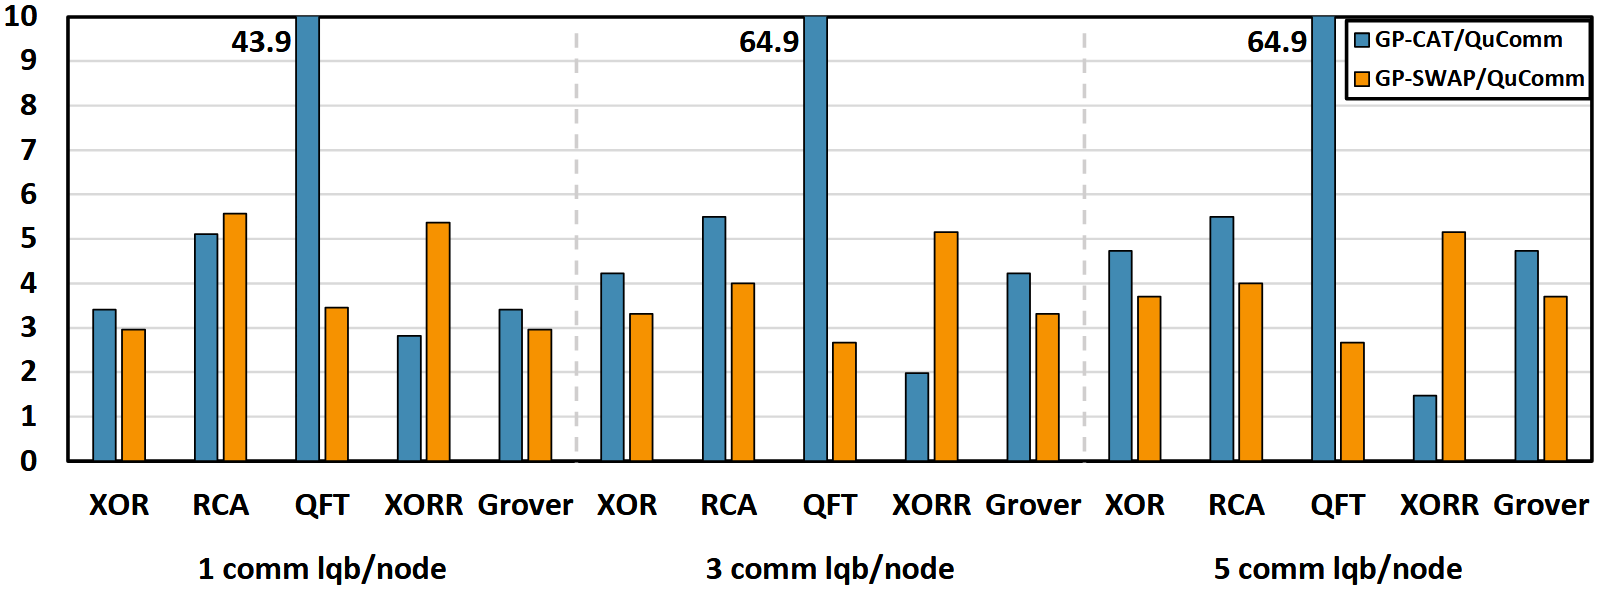
\includegraphics[width=.8\textwidth]{figure/other.png}
			\caption[]{QuComm achieves up to 5× fewer inter-node communications compared to GP-CAT and GP-SWAP. Collective block optimization enables large communication savings that simpler burst-based or SWAP-based methods cannot match.}
		\end{figure}
	\end{frame}
	
	\begin{frame}{Architecture Adaptability}
		\begin{figure}
			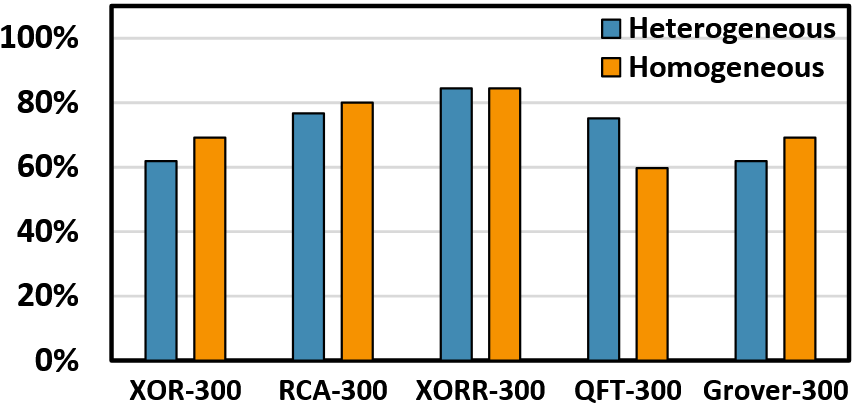
\includegraphics[width=0.4\textwidth]{figure/ad-1.png}
			\hspace*{4pt}
			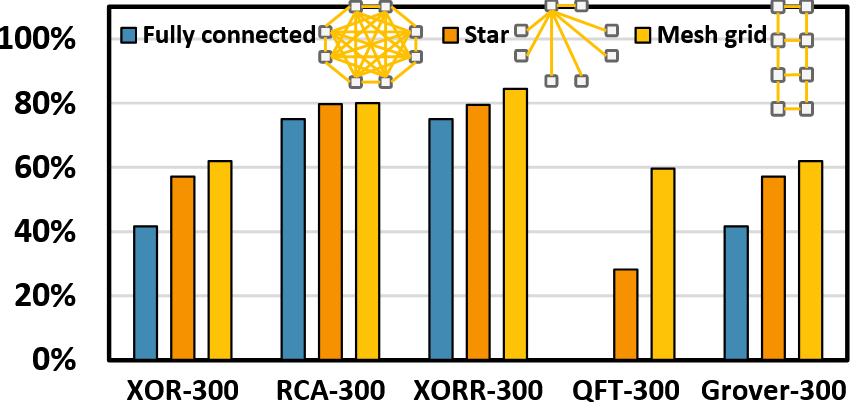
\includegraphics[width=0.4\textwidth]{figure/ad-2.png}
			\caption[]{QuComm remains effective across topologies and node sizes.}
		\end{figure}
		\begin{itemize}
			\item Works on mesh, star, and full networks.
			\item Robust to node heterogeneity.
			\item Collective optimization generalizes well.
		\end{itemize}
	\end{frame}
	
	\begin{frame}{Conclusion}
		\begin{itemize}
			\item QuComm uncovers hidden multi-node patterns.
			\item Substantially reduces inter-node gate count.
			\item Enables scalable DQC with limited hardware.
%			\item Future: integrate with QEC, runtime compilers, cloud workloads.
		\end{itemize}
	\end{frame}
	
\end{document}
